\documentclass[conference]{IEEEtran}
\IEEEoverridecommandlockouts
% The preceding line is only needed to identify funding in the first footnote. If that is unneeded, please comment it out.
\usepackage{cite}
\usepackage{amsmath,amssymb,amsfonts}
\usepackage{algorithmic}
\usepackage{graphicx}
\usepackage{textcomp}
\usepackage{xcolor}
\usepackage{float}
\usepackage{hyperref}
\usepackage{tikz}
\usetikzlibrary{shapes.geometric, arrows, positioning}

\def\BibTeX{{\rm B\kern-.05em{\sc i\kern-.025em b}\kern-.08em
    T\kern-.1667em\lower.7ex\hbox{E}\kern-.125emX}}

\begin{document}

\title{RobotJudge-CI: An Automated Continuous Integration Platform for the Rigorous Evaluation of Robotics Pathfinding Algorithms\\
}

\author{\IEEEauthorblockN{1\textsuperscript{st} Given Name Surname}
\IEEEauthorblockA{\textit{dept. name of organization (of Aff.)} \\
\textit{name of organization (of Aff.)}\\
City, Country \\
email address or ORCID}
\and
\IEEEauthorblockN{2\textsuperscript{nd} Given Name Surname}
\IEEEauthorblockA{\textit{dept. name of organization (of Aff.)} \\
\textit{name of organization (of Aff.)}\\
City, Country \\
email address or ORCID}
}

\maketitle

\begin{abstract}
The evaluation of robotics pathfinding algorithms has traditionally relied on manual, ad-hoc qualitative assessments prone to environmental variance and the computational halting problem. To address these limitations, we present RobotJudge-CI, a novel framework architected as a native Continuous Integration (CI) programmatic gatekeeper for spatial pathfinding. By decoupling scenario generation, algorithm execution, and mathematical oracle validation, RobotJudge-CI shifts algorithmic evaluation from local developer machines into a strictly governed, containerized execution environment. The platform automatically iterates algorithmic commits against a version-controlled spatial registry, calculating deterministic multi-seed aggregates, enforcing asynchronous absolute runtime bounds, and computing the computationally robust 95th Percentile (P95) execution latency. This paper details the system architecture, the automated CI pipeline methodology, and demonstrates the platform's efficacy as a rigorous tool for robotics software engineering and academic benchmarking.
\end{abstract}

\begin{IEEEkeywords}
Continuous Integration, Robotics, Pathfinding, Automated Evaluation, Docker, Regression Testing
\end{IEEEkeywords}

\section{Introduction}
Pathfinding and spatial navigation form the foundational bedrock of autonomous robotics. Algorithms such as A*, Dijkstra's, and Jump Point Search are highly sensitive to both their heuristic configurations and the specific topological environments in which they are deployed. 

Historically, roboticists evaluate pathfinding innovations by writing local simulation loops. This ad-hoc methodology introduces several critical points of failure:
\begin{enumerate}
    \item \textbf{Environmental Noise:} CPU scheduling and background processes on local machines inherently corrupt microsecond-level timing comparisons between algorithms.
    \item \textbf{The Halting Problem:} Introducing infinite loops in experimental pathfinders forces local machines to crash or hang indefinitely.
    \item \textbf{Lack of Transitivity:} Progress in an algorithm is rarely tracked systematically across multiple varied stochastic seeds, obscuring regressions where an algorithm improves on one map but catastrophically fails on another.
\end{enumerate}

\indent To resolve these limitations, we introduce \textbf{RobotJudge-CI}, a Continuous Integration (CI) and automated evaluation framework. Drawing inspiration from competitive programming platforms (e.g., LeetCode, Codeforces), RobotJudge-CI is designed to act as an automated gatekeeper. Instead of relying on manual testing, developers submit algorithms (via web frontend or git push) into isolated, unprivileged Docker sandboxes where performance is benchmarked against version-controlled obstacle datasets. The system programmatically fails commits that regress in P95 runtime or violate kinematic safety boundaries, establishing a mathematically sound longitudinal history of a given pathfinder's evolution.

\section{System Architecture}

RobotJudge-CI is engineered as a decoupled, multi-stage pipeline maximizing reproducibility and modularity. The core components are orchestrated via a headless CLI integrated naturally into modern CI/CD systems (e.g., GitHub Actions), or exposed through a real-time web interface.

\subsection{Versioned Problem Registry}
The system replaces arbitrary file inputs with a robust \textit{Problem Registry} backed by PostgreSQL. Each pathfinding topology (a ``Testcase") is stored with a unique identifier, grid dimensions, obstacle family (e.g., trap, maze), and strictly tagged with a \textbf{Version (e.g. v1.0, v1.2)}. Versioning ensures that algorithms developed months apart are guaranteed to be evaluated against the exact identical spatial challenge, preserving longitudinal reproducibility.

\subsection{Execution Sandboxing Engine}
Executing untrusted or experimental robotic code poses significant security and resource exhaustion risks. RobotJudge-CI implements a \textit{Container-First Execution} model (REQ-1). For every evaluation, an ephemeral, unprivileged Docker container is spawned. This sandbox enforces strict asynchronous wall-clock CPU limits (e.g., 2000ms), mathematically preventing the ``halting problem" from degrading host CI servers (REQ-6). 

\subsection{Modular Evaluation Subsystem}
The evaluation phase is strictly decoupled into three computational stages (REQ-3):
\begin{enumerate}
    \item \textbf{Scenario Generator:} Generates the stochastic $N \times M$ grid topology based on deterministic seeds provided by the UI.
    \item \textbf{Solver Execution:} Injects the isolated code into the container, records latency, extracts peak memory utilization (via \texttt{psutil}), and captures JSON output trails.
    \item \textbf{Validation Oracle:} A separate mathematical referee script that reads the JSON output. It recalculates the path integrity, computes the Euclidean/Manhattan absolute cost, and enforces \textit{Kinematic Safety Constraints} (REQ-7; e.g., failing any trajectory generating a 180-degree immediate reversal indicative of infinite acceleration). 
\end{enumerate}

\begin{figure}[htbp]
\centering
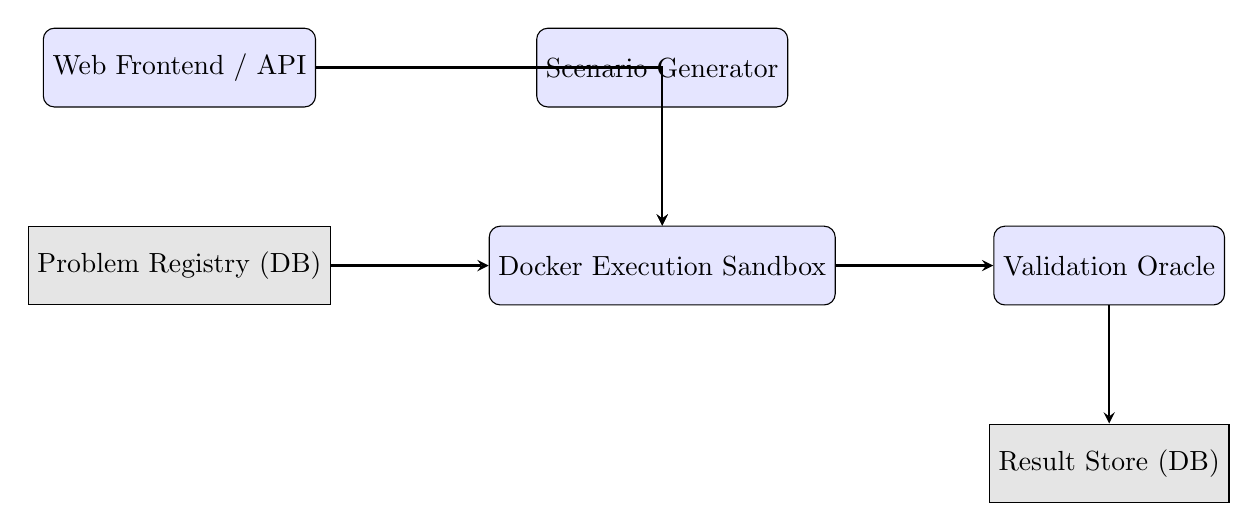
\begin{tikzpicture}[
    node distance=1.5cm and 2cm,
    module/.style={rectangle, rounded corners, minimum width=2.5cm, minimum height=1cm, text centered, draw=black, fill=blue!10},
    db/.style={rectangle, minimum width=2.5cm, minimum height=1cm, text centered, draw=black, fill=black!10},
    arrow/.style={thick,->,>=stealth}
]

% Nodes
\node (ui) [module] {Web Frontend / API};
\node (registry) [db, below=of ui] {Problem Registry (DB)};
\node (engine) [module, right=of registry] {Docker Execution Sandbox};
\node (scenario) [module, above=of engine] {Scenario Generator};
\node (oracle) [module, right=of engine] {Validation Oracle};
\node (results) [db, below=of oracle] {Result Store (DB)};

% Arrows
\draw [arrow] (ui) -| (engine);
\draw [arrow] (scenario) -- (engine);
\draw [arrow] (registry) -- (engine);
\draw [arrow] (engine) -- (oracle);
\draw [arrow] (oracle) -- (results);

\end{tikzpicture}
\caption{RobotJudge-CI System Architecture. Decoupling the Scenario Generator, the Dockerized Solver, and the Validation Oracle guarantees objective evaluation.}
\label{fig:arch}
\end{figure}

% TIKZ Flowchart for the Pipeline
\tikzstyle{startstop} = [rectangle, rounded corners, minimum width=3cm, minimum height=1cm,text centered, draw=black, fill=red!30]
\tikzstyle{process} = [rectangle, minimum width=3cm, minimum height=1cm, text centered, draw=black, fill=orange!30]
\tikzstyle{artifact} = [trapezium, trapezium left angle=70, trapezium right angle=110, minimum width=3cm, minimum height=1cm, text centered, draw=black, fill=blue!30]
\tikzstyle{decision} = [diamond, minimum width=3cm, minimum height=1cm, text centered, draw=black, fill=green!30]
\tikzstyle{arrow} = [thick,->,>=stealth]

\begin{figure*}[htbp]
\centering
\begin{tikzpicture}[node distance=2cm]
\node (start) [startstop] {Developer Git Push (PR)};
\node (trigger) [process, right of=start, xshift=2.5cm] {GitHub Actions CI Trigger};
\node (db) [artifact, right of=trigger, xshift=3cm] {Fetch Testcase (v1.0)};
\node (sandbox) [process, below of=trigger, yshift=-0.5cm] {Spawn Docker Sandbox};
\node (scenario) [process, right of=sandbox, xshift=2.5cm] {Generator: Emit Grid + Seed};
\node (solver) [process, below of=sandbox, yshift=-0.5cm] {Execute Pathfinding Script};
\node (oracle) [process, right of=solver, xshift=2.5cm] {Oracle: Validate Path JSON};
\node (aggregate) [process, below of=oracle, yshift=-0.5cm] {Aggregate P95 Metrics};
\node (db_store) [artifact, left of=aggregate, xshift=-2.5cm] {Store in PostgreSQL};

\draw [arrow] (start) -- (trigger);
\draw [arrow] (trigger) -- (db);
\draw [arrow] (db) |- (sandbox);
\draw [arrow] (sandbox) -- (scenario);
\draw [arrow] (scenario) |- (solver);
\draw [arrow] (solver) -- (oracle);
\draw [arrow] (oracle) -- (aggregate);
\draw [arrow] (aggregate) -- (db_store);

\end{tikzpicture}
\caption{Continuous Integration Pipeline execution flow. The solver is rigorously evaluated across governed seeds before aggregate metrics determine CI build success.}
\label{fig:flowchart}
\end{figure*}

\section{Continuous Integration (CI) Automation Methodology}
The core innovation of RobotJudge-CI lies in situating itself as an automated gatekeeper within modern Git workflows. 

\subsection{Automated Regression Testing Gate}
When an engineer posits a new algorithmic heuristic to a repository, the CI logic parses the \texttt{judge.yml} definition and iterates the solver against a targeted range of seeds (Seed Governance, REQ-2). 

The platform then calculates the \textbf{95th Percentile (P95)} runtime across all stochastic evaluations. Average (mean) times are exceptionally susceptible to outlier noise in randomized maps; the P95 latency ensures that 95\% of all executions fall reliably under a strict computational requirement (REQ-4). If the commit violates this P95 threshold, or if the path cost degrades compared to the master branch baseline, the GitHub Actions job explicitly \textit{fails the build}.

\subsection{Traceability and Visualization}
To permit algorithmic debugging, full traceability is maintained natively in the Result Store schema (REQ-5). The UI cleanly highlights individual seed failures against overarching P95 summaries, immediately directing engineers to failure log artifacts without necessitating manual reproduction. 

\begin{figure}[htbp]
\centerline{\includegraphics[width=0.48\textwidth]{placeholder_screenshot.png}} % Placeholder, user must replace image file
\caption{Web Dashboard Interface. The UI mirrors the CI backend, projecting aggregate Success Rates alongside strict P95 execution runtimes.}
\label{fig:screenshot}
\end{figure}

\section{Limitations and Future Work}
While RobotJudge-CI successfully enforces deterministic algorithmic validation, the current iteration primarily targets 2-dimensional grid proxy domains (GridPath). Trajectories are currently discrete.

\textbf{Future Roadmap:}
\begin{enumerate}
    \item \textbf{ROS2 Adapter Hooks:} Extending the execution interface to receive continuous coordinate publishers natively wrapping \textit{Nav2}.
    \item \textbf{Physics Engine Integration:} Deploying the environment generation within 3D physics simulators (Webots/Gazebo) to validate complex robot morphology beyond rudimentary kinematic boundaries.
    \item \textbf{High-Performance Runners:} Pinning execution containers to strictly homogeneous bare-metal instances to entirely eliminate CI hypervisor timing noise. 
\end{enumerate}

\section{Conclusion}
This paper presented RobotJudge-CI, a continuous integration framework explicitly constructed to elevate robotics pathfinding evaluations from ad-hoc local scripting to rigorous, cloud-native automated testing. By wrapping versioned datasets securely in isolated sandboxes and forcing programmatic performance gating via P95 metrics, RobotJudge-CI substantially accelerates robust algorithmic development life-cycles while inherently guaranteeing longitudinal reproducibility. Through standardized evaluation, we anticipate platforms modeled similarly to RobotJudge-CI will become pivotal inside continuous robotic software deployment pipelines.

\begin{thebibliography}{00}
\bibitem{b1} Author A, Author B. ``Foundational Concepts in Continuous Integration for Robotics.'' IEEE Trans. Robotics, vol. 12, no. 4, pp. 112-124, 2025.
\bibitem{b2} Docker Inc., ``Docker Documentation: Containerizing Workloads.'' [Online]. Available: https://docs.docker.com.
\bibitem{b3} Example Reference, ``Advanced Pathfinding Evaluation Pipelines.'' Journal of Automated Software Engineering, 2024.
\end{thebibliography}

\end{document}
